\documentclass[11pt,a4paper]{report}
\usepackage[textwidth=37em,vmargin=30mm]{geometry}
\usepackage{calc,xunicode,amsmath,amssymb,paralist,enumitem,tabu,booktabs,datetime2,xeCJK,xeCJKfntef,listings}
\usepackage{tocloft,fancyhdr,tcolorbox,xcolor,graphicx,eso-pic,xltxtra,xelatexemoji}

\newcommand{\envyear}[0]{2025}
\newcommand{\envdatestr}[0]{2025-08-26}
\newcommand{\envfinaldir}[0]{webdb/2025/20250826/final}

\usepackage[hidelinks]{hyperref}
\hypersetup{
    colorlinks=false,
    pdfpagemode=FullScreen,
    pdftitle={Web Digest - \envdatestr}
}

\setlength{\cftbeforechapskip}{10pt}
\renewcommand{\cftchapfont}{\rmfamily\bfseries\large\raggedright}
\setlength{\cftbeforesecskip}{2pt}
\renewcommand{\cftsecfont}{\sffamily\small\raggedright}

\setdefaultleftmargin{2em}{2em}{1em}{1em}{1em}{1em}

\usepackage{xeCJK,xeCJKfntef}
\xeCJKsetup{PunctStyle=plain,RubberPunctSkip=false,CJKglue=\strut\hskip 0pt plus 0.1em minus 0.05em,CJKecglue=\strut\hskip 0.22em plus 0.2em}
\XeTeXlinebreaklocale "zh"
\XeTeXlinebreakskip = 0pt


\setmainfont{Brygada 1918}
\setromanfont{Brygada 1918}
\setsansfont{IBM Plex Sans}
\setmonofont{JetBrains Mono NL}
\setCJKmainfont{Noto Serif CJK SC}
\setCJKromanfont{Noto Serif CJK SC}
\setCJKsansfont{Noto Sans CJK SC}
\setCJKmonofont{Noto Sans CJK SC}

\setlength{\parindent}{0pt}
\setlength{\parskip}{8pt}
\linespread{1.15}

\lstset{
	basicstyle=\ttfamily\footnotesize,
	numbersep=5pt,
	backgroundcolor=\color{black!5},
	showspaces=false,
	showstringspaces=false,
	showtabs=false,
	tabsize=2,
	captionpos=b,
	breaklines=true,
	breakatwhitespace=true,
	breakautoindent=true,
	linewidth=\textwidth
}






\newcommand{\coverpic}[2]{
    % argv: itemurl, authorname
    Cover photo by #2~~(\href{#1}{#1})
}
\newcommand{\makeheader}[0]{
    \begin{titlepage}
        % \newgeometry{hmargin=15mm,tmargin=21mm,bmargin=12mm}
        \begin{center}
            
            \rmfamily\scshape
            \fontspec{BaskervilleF}
            \fontspec{Old Standard}
            \fontsize{59pt}{70pt}\selectfont
            WEB\hfill DIGEST
            
            \vfill
            % \vskip 30pt
            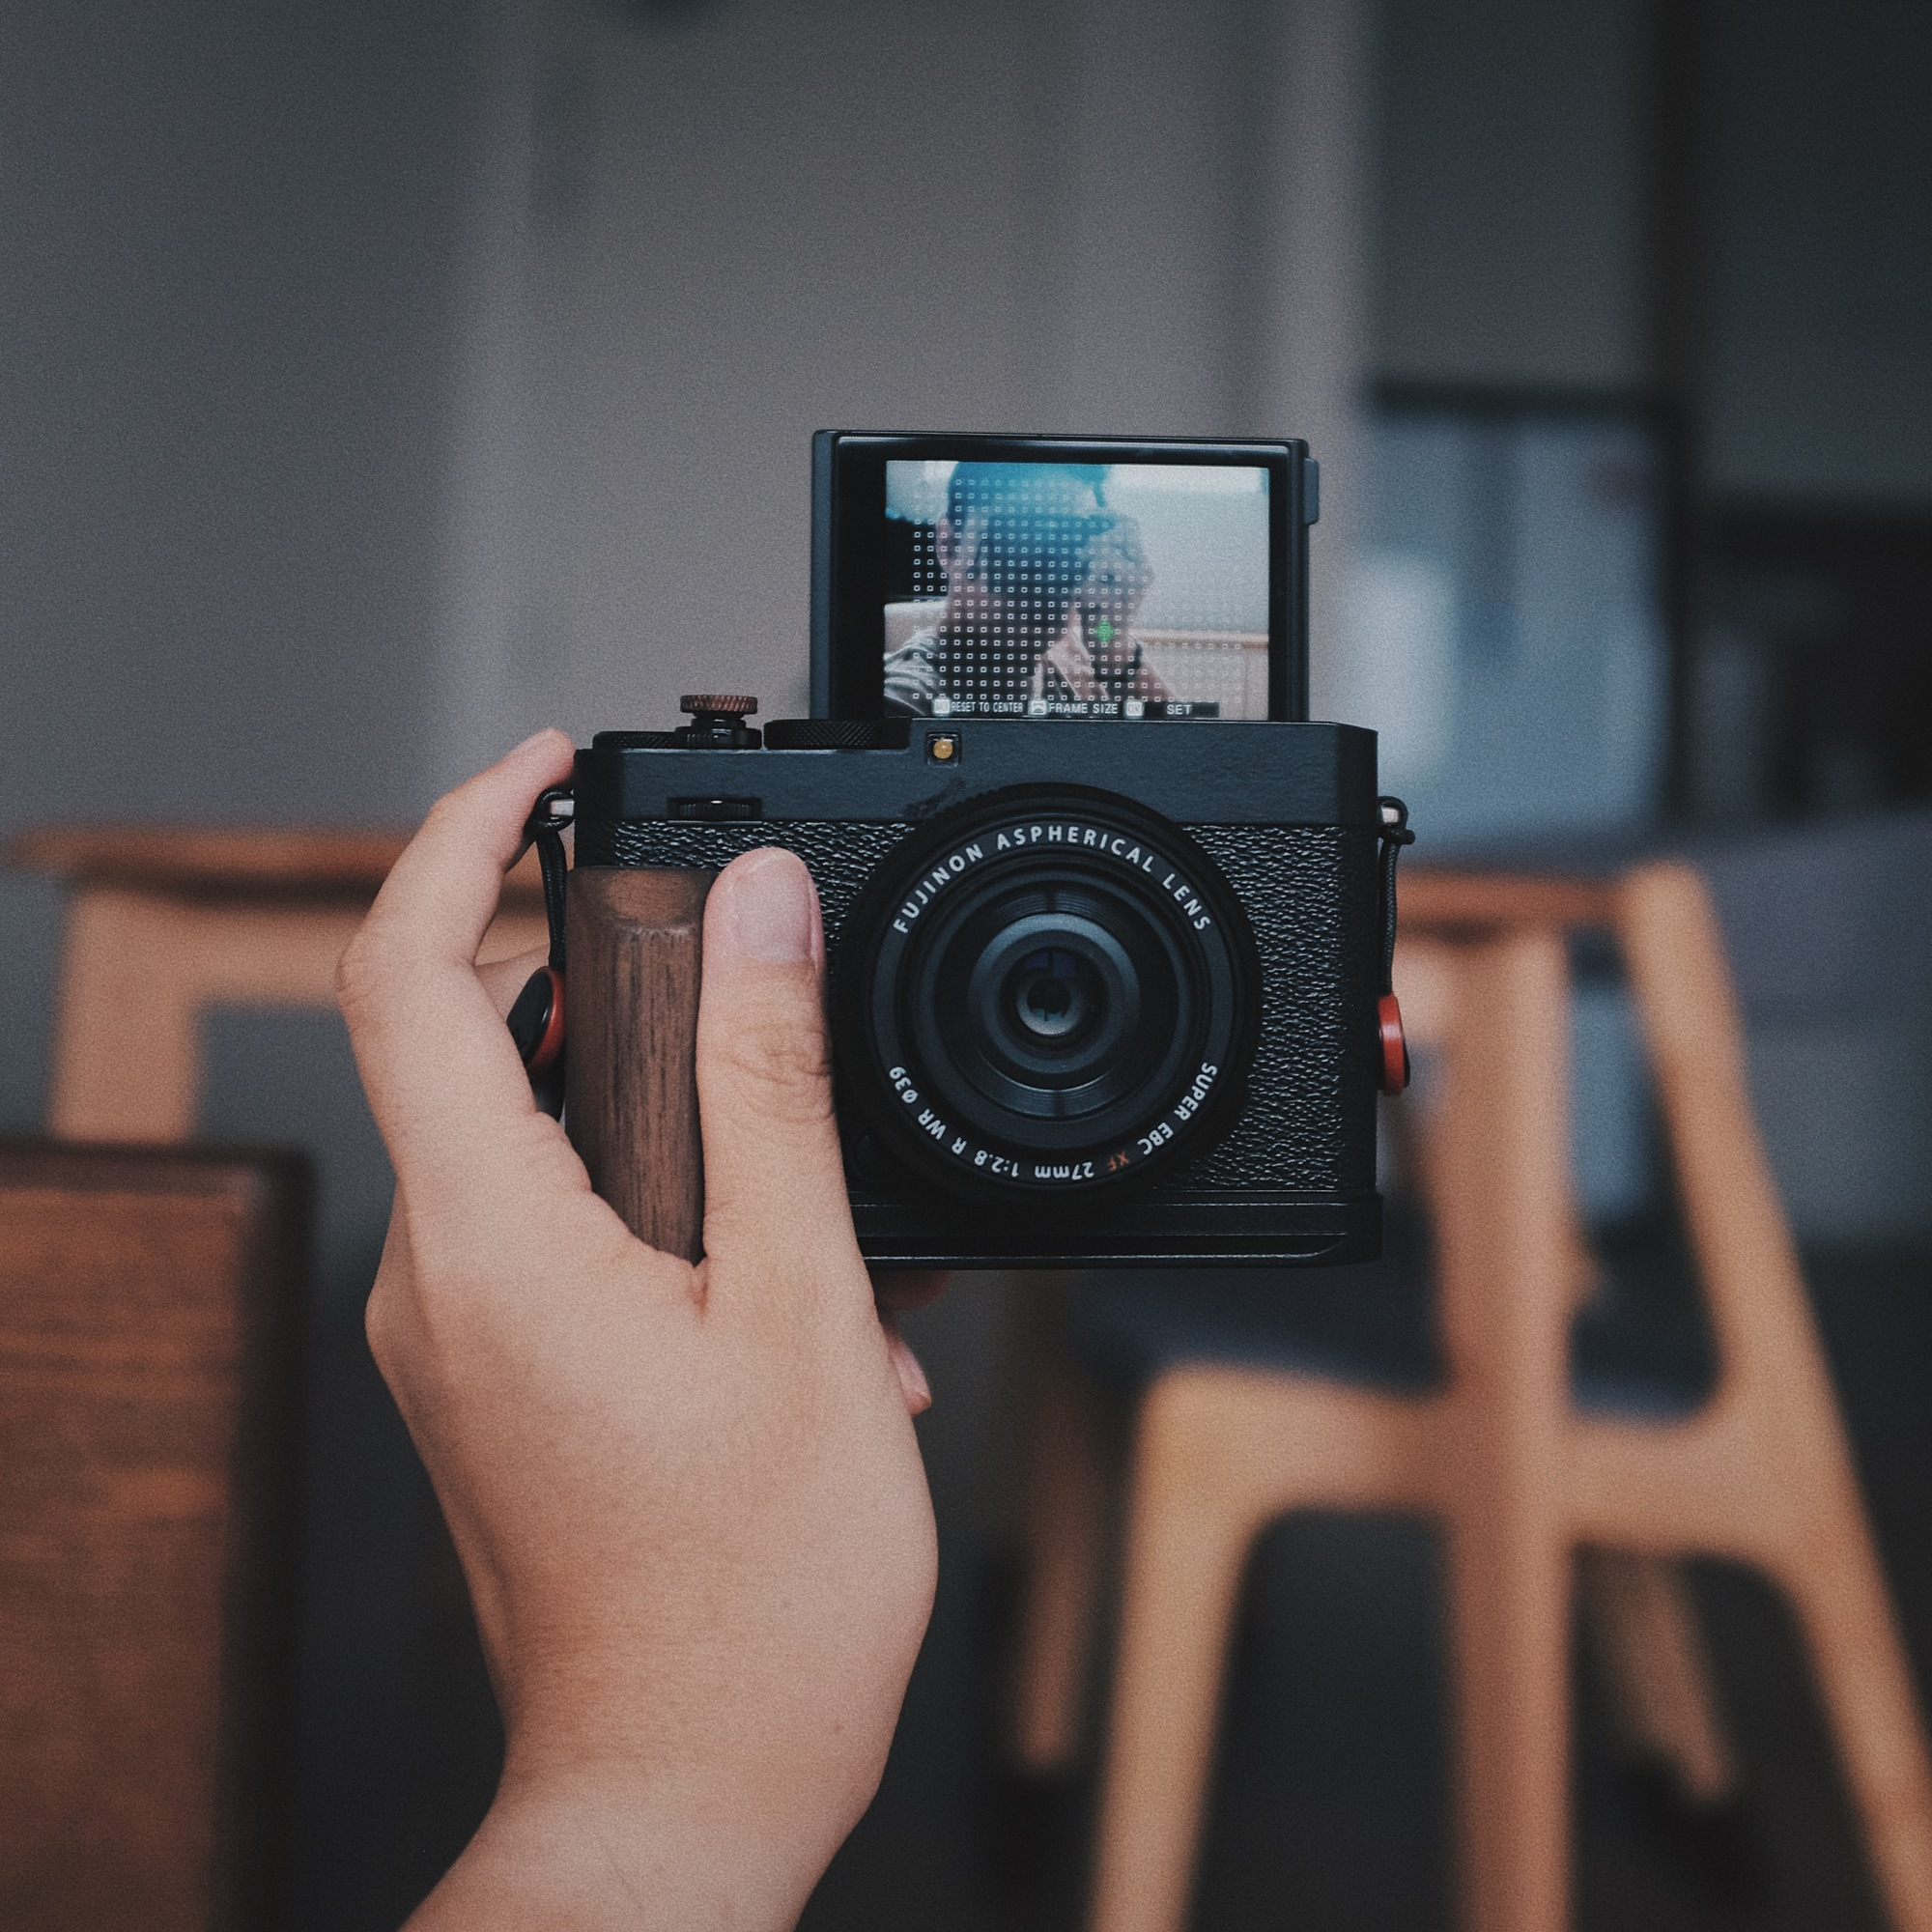
\includegraphics[width=\linewidth]{\envfinaldir/coverpic-prod.jpg}\par
            % \vskip 30pt
            \vfill

            \normalsize\rmfamily\scshape
            \copyright{} The Web Digest Project \hfill\large \envdatestr
        \end{center}
    \end{titlepage}
    % \restoregeometry
}
\newcommand{\simplehref}[1]{%
    \textcolor{blue!80!green}{\href{#1}{#1}}%
}
\renewcommand{\contentsname}{\center\Huge\sffamily\bfseries Contents\par\vskip 20pt}
\newcounter{ipartcounter}
\setcounter{ipartcounter}{0}
\newcommand{\ipart}[1]{
    % \vskip 20pt
    \clearpage
    \stepcounter{ipartcounter}
    \phantomsection
    \addcontentsline{toc}{chapter}{#1}
    % \begin{center}
    %     \Huge
    %     \sffamily\bfseries
    %     #1
    % \end{center}
    % \vskip 20pt plus 7pt
}
\newcounter{ichaptercounter}
\setcounter{ichaptercounter}{0}
\newcommand{\ichapter}[1]{
    % \vskip 20pt
    \clearpage
    \stepcounter{ichaptercounter}
    \phantomsection
    \addcontentsline{toc}{section}{\numberline{\arabic{ichaptercounter}}#1}
    \begin{center}
        \Huge
        \sffamily\bfseries
        #1
    \end{center}
    \vskip 20pt plus 7pt
}
\newcommand{\entrytitlefont}[1]{\subsection*{\raggedright\Large\sffamily\bfseries#1}}
\newcommand{\entryitemGeneric}[2]{
    % argv: title, url
    \parbox{\linewidth}{
        \entrytitlefont{#1}\par\vskip 5pt
        \footnotesize\ttfamily\mdseries
        \simplehref{#2}
    }\vskip 11pt plus 11pt minus 1pt
}
\newcommand{\entryitemGithub}[3]{
    % argv: title, url, desc
    \parbox{\linewidth}{
        \entrytitlefont{#1}\par\vskip 5pt
        \footnotesize\ttfamily\mdseries
        \simplehref{#2}\par\vskip 5pt
        \small\rmfamily\mdseries#3
    }\vskip 11pt plus 11pt minus 1pt
}
\newcommand{\entryitemAp}[3]{
    % argv: title, url, desc
    \parbox{\linewidth}{
        \entrytitlefont{#1}\par\vskip 5pt
        \footnotesize\ttfamily\mdseries
        \simplehref{#2}\par\vskip 5pt
        \small\rmfamily\mdseries#3
    }\vskip 11pt plus 11pt minus 1pt
}
\newcommand{\entryitemHackernews}[3]{
    % argv: title, hnurl, rawurl
    % \parbox{\linewidth}{
    %     \entrytitlefont{#1}\par\vskip 5pt
    %     \footnotesize\ttfamily\mdseries
    %     \simplehref{#3}\par
    %     \textcolor{black!50}{\href{#2}{#2}}
    % }\vskip 11pt plus 11pt minus 1pt
    \begin{minipage}{\linewidth}
            \entrytitlefont{#1}\par\vskip 5pt
            \footnotesize\ttfamily\mdseries
            \simplehref{#3}\par
            \textcolor{black!50}{\href{#2}{#2}}
    \end{minipage}\par\vskip 11pt plus 11pt minus 1pt
}







\begin{document}

\makeheader

\tableofcontents\clearpage




\ipart{Developers}
\ichapter{Hacker News}
\entryitemTwoLinks{Google to require developer verification for Android apps outside the Play Store}{https://news.ycombinator.com/item?id=45018343}{https://techcrunch.com/2025/08/25/google-will-require-developer-verification-for-android-apps-outside-the-play-store/}

\entryitemTwoLinks{Meta just suspended the Facebook account of Neal Stephenson}{https://news.ycombinator.com/item?id=45017969}{https://twitter.com/nealstephenson/status/1959759051732213812}

\entryitemTwoLinks{Google to require developer verification to install and sideload Android apps}{https://news.ycombinator.com/item?id=45017028}{https://9to5google.com/2025/08/25/android-apps-developer-verification/}

\entryitemTwoLinks{Google's Liquid Cooling}{https://news.ycombinator.com/item?id=45016720}{https://chipsandcheese.com/p/googles-liquid-cooling-at-hot-chips}

\entryitemTwoLinks{Temporary suspension of acceptance of mail to the United States}{https://news.ycombinator.com/item?id=45016517}{https://www.post.japanpost.jp/int/information/2025/0825\_01\_en.html}

\entryitemTwoLinks{The MiniPC Revolution}{https://news.ycombinator.com/item?id=45015814}{https://jadarma.github.io/blog/posts/2025/08/the-minipc-revolution/}

\entryitemTwoLinks{FCC bars providers for non-compliance with robocall protections}{https://news.ycombinator.com/item?id=45015354}{https://docs.fcc.gov/public/attachments/DOC-414073A1.txt}

\entryitemTwoLinks{Building the mouse Logitech won't make}{https://news.ycombinator.com/item?id=45014993}{https://samwilkinson.io/posts/2025-08-24-mx-ergo-mods}

\entryitemTwoLinks{Hundreds lose water source in Colorado's poorest county with no notice}{https://news.ycombinator.com/item?id=45014489}{https://coloradosun.com/2025/08/25/costilla-county-water-cutoff/}

\entryitemTwoLinks{Show HN: Base, an SQLite database editor for macOS}{https://news.ycombinator.com/item?id=45014131}{https://menial.co.uk/base/}

\entryitemTwoLinks{Japan's Creepiest Station}{https://news.ycombinator.com/item?id=45013774}{https://www.tokyocowboy.co/articles/doai-eki-japans-creepiest-station}

\entryitemTwoLinks{A small change to improve browsers for keyboard navigation}{https://news.ycombinator.com/item?id=45013737}{https://b.43z.one/2025-07-22/}

\entryitemTwoLinks{The unlikely revival of nuclear batteries}{https://news.ycombinator.com/item?id=45013714}{https://spectrum.ieee.org/nuclear-battery-revival}

\entryitemTwoLinks{What is a color space?}{https://news.ycombinator.com/item?id=45013154}{https://www.makingsoftware.com/chapters/color-spaces-models-and-gamuts}

\entryitemTwoLinks{An illustrated guide to OAuth}{https://news.ycombinator.com/item?id=45013131}{https://www.ducktyped.org/p/an-illustrated-guide-to-oauth}

\entryitemTwoLinks{Standard Thermal: Energy Storage 500x Cheaper Than Batteries}{https://news.ycombinator.com/item?id=45012942}{https://austinvernon.site/blog/standardthermal.html}

\entryitemTwoLinks{The Size of Adobe Reader Installers Through the Years}{https://news.ycombinator.com/item?id=45012931}{https://sigwait.org/~alex/blog/2025/08/25/zw6z4E.html}

\entryitemTwoLinks{Agent-C: a 4KB AI agent}{https://news.ycombinator.com/item?id=45012430}{https://github.com/bravenewxyz/agent-c}

\entryitemTwoLinks{Scamlexity: When agentic AI browsers get scammed}{https://news.ycombinator.com/item?id=45011096}{https://guard.io/labs/scamlexity-we-put-agentic-ai-browsers-to-the-test-they-clicked-they-paid-they-failed}

\entryitemTwoLinks{What are OKLCH colors?}{https://news.ycombinator.com/item?id=45010876}{https://jakub.kr/components/oklch-colors}\ichapter{Phoronix}
\entryitemGeneric{\hskip 0pt{}Linux's Floppy Disk Driver Code Sees Some Cleanups In 2025}{https://www.phoronix.com/news/Linux-Floppy-Disk-Cleanups-2025}

\entryitemGeneric{\hskip 0pt{}Linux 5.15 LTS To 6.17 Benchmarks: Four Years Of Kernel Improvement Net 37\% Improvement On AMD EPYC}{https://www.phoronix.com/review/linux-515-617-performance}

\entryitemGeneric{\hskip 0pt{}Red Hat Releases TuneD 2.26 For Adaptively Tuning Linux Systems}{https://www.phoronix.com/news/Red-Hat-TuneD-2.26}

\entryitemGeneric{\hskip 0pt{}Meson 1.9 Released With New Rust Features, Adds Swift/C++ Interoperability}{https://www.phoronix.com/news/Meson-1.9-Released}

\entryitemGeneric{\hskip 0pt{}Open Platform For Enterprise AI's GenAI Code Adds Guardrails, AMD EPYC Support}{https://www.phoronix.com/news/OPEA-1.4-Gen-AI-Released}

\entryitemGeneric{\hskip 0pt{}Linux 6.18 Will Begin Preparing For ASPEED AST2700 BMC Support}{https://www.phoronix.com/news/ASPEED-AST2700-Linux-6.18}

\entryitemGeneric{\hskip 0pt{}Linux Foundation Forms The Developer Relations Foundation, DocumentDB Joins The LF}{https://www.phoronix.com/news/Linux-Foundation-DRF}

\entryitemGeneric{\hskip 0pt{}Linux 6.17-rc3 Released: "A Bit Larger Than Usual"}{https://www.phoronix.com/news/Linux-6.17-rc3-Released}

\entryitemGeneric{\hskip 0pt{}CachyOS Introduces Packages Dashboard, GRUB+Btrfs Bootable Snapshots}{https://www.phoronix.com/news/CachyOS-August-2025}


\ipart{Developers~~~~(zh-Hans)}
\ichapter{Solidot}
\entryitemGeneric{\hskip 0pt{}谷神星可能曾经宜居}{https://www.solidot.org/story?sid=82135}

\entryitemGeneric{\hskip 0pt{}小肯尼迪要求撤回一篇疫苗研究论文,期刊拒绝}{https://www.solidot.org/story?sid=82134}

\entryitemGeneric{\hskip 0pt{}新西兰空管系统因软件故障罢工一小时}{https://www.solidot.org/story?sid=82133}

\entryitemGeneric{\hskip 0pt{}张益唐称他因为政治气候从美国回到中国}{https://www.solidot.org/story?sid=82132}

\entryitemGeneric{\hskip 0pt{}为前雇主 IT 系统设立关闭开关的开发者被判四年}{https://www.solidot.org/story?sid=82131}

\entryitemGeneric{\hskip 0pt{}OpenAI 用 Google 搜索数据挑战 Google}{https://www.solidot.org/story?sid=82130}

\entryitemGeneric{\hskip 0pt{}Google TV 和 Android TV 应用到 2026 年 8 月都必须支持 64 位}{https://www.solidot.org/story?sid=82129}

\entryitemGeneric{\hskip 0pt{}英特尔同意美国政府控制 10\% 股份}{https://www.solidot.org/story?sid=82128}

\entryitemGeneric{\hskip 0pt{}FFmpeg 8.0 释出}{https://www.solidot.org/story?sid=82127}

\entryitemGeneric{\hskip 0pt{}Arch Linux 遭遇 DDoS 攻击}{https://www.solidot.org/story?sid=82126}

\entryitemGeneric{\hskip 0pt{}Google 数据中心的用水量}{https://www.solidot.org/story?sid=82125}\ichapter{V2EX}
\entryitemGeneric{\hskip 0pt{}[分享发现] 杭州通上线 applepay 了}{https://www.v2ex.com/t/1154897}

\entryitemGeneric{\hskip 0pt{}[macOS] macos26 beta8 的聚焦搜索的内存泄漏解决了吗}{https://www.v2ex.com/t/1154896}

\entryitemGeneric{\hskip 0pt{}[生活] 大家有啥精简做饭的技巧吗?}{https://www.v2ex.com/t/1154894}

\entryitemGeneric{\hskip 0pt{}[分享创造] 强推 AdonisJS 我为他开发了一个 dcat/laravel-admin 平替后台面板 EaseAdmin}{https://www.v2ex.com/t/1154892}

\entryitemGeneric{\hskip 0pt{}[生活] 我还要继续吗?}{https://www.v2ex.com/t/1154890}

\entryitemGeneric{\hskip 0pt{}[Safari] macOS 15 上 Safari 怎么很卡}{https://www.v2ex.com/t/1154889}

\entryitemGeneric{\hskip 0pt{}[问与答] [求大神指导] 投资 400w 的酒店,月营收 7w+,有点经营不下去了,转让 or 破局?}{https://www.v2ex.com/t/1154888}

\entryitemGeneric{\hskip 0pt{}[Bing] bing 国内版竟然搜不到 site:cloudflare.com,只能搜到 cloudflare-cn.com}{https://www.v2ex.com/t/1154887}

\entryitemGeneric{\hskip 0pt{}[Node.js] adonisjs 有没有现成的注册登录库?}{https://www.v2ex.com/t/1154886}

\entryitemGeneric{\hskip 0pt{}[程序员] 之前一直用 SonarQube 做代码审计,现在 ai 这么发达有什么好用的代码审计工具吗,主要语言是 go}{https://www.v2ex.com/t/1154885}

\entryitemGeneric{\hskip 0pt{}[投资] macos 炒股这么痛苦吗?}{https://www.v2ex.com/t/1154884}

\entryitemGeneric{\hskip 0pt{}[NAS] 各位来分享一下自己的个人数据备份方案吧}{https://www.v2ex.com/t/1154883}

\entryitemGeneric{\hskip 0pt{}[问与答] 国内建站推荐}{https://www.v2ex.com/t/1154881}

\entryitemGeneric{\hskip 0pt{}[生活] 候补了一张邓紫棋的票,搜了下她的身世,果然五世家业才有的黄四郎}{https://www.v2ex.com/t/1154880}

\entryitemGeneric{\hskip 0pt{}[杭州] 房子该不该卖了}{https://www.v2ex.com/t/1154878}

\entryitemGeneric{\hskip 0pt{}[Apple] 头疼! macOS 更新后显示器内置拓展坞不工作}{https://www.v2ex.com/t/1154877}

\entryitemGeneric{\hskip 0pt{}[酷工作] [内推] [校招] [机器人公司] [深圳/成都]}{https://www.v2ex.com/t/1154876}

\entryitemGeneric{\hskip 0pt{}[程序员] 密码的,外包强度怎么这么高}{https://www.v2ex.com/t/1154875}

\entryitemGeneric{\hskip 0pt{}[分享发现] 如果你去白俄罗斯明斯克玩,或许用得着这个网站}{https://www.v2ex.com/t/1154874}

\entryitemGeneric{\hskip 0pt{}[随想] 疑似只有我用的第一款手机是努比亚}{https://www.v2ex.com/t/1154873}

\entryitemGeneric{\hskip 0pt{}[加密货币] 游戏搬砖弄了 250 多 usdt 请问下怎么出?}{https://www.v2ex.com/t/1154872}

\entryitemGeneric{\hskip 0pt{}[投资] 美股 Nvidia/TSM 买入/卖出还是观望?}{https://www.v2ex.com/t/1154871}

\entryitemGeneric{\hskip 0pt{}[程序员] 小工具预热 MCP 功能即将推出 [域名各种指标,流量趋势,反向链接]}{https://www.v2ex.com/t/1154870}

\entryitemGeneric{\hskip 0pt{}[App Store] 大家在 appstore 应用商店 macos 的预览图是怎么生成的呢?}{https://www.v2ex.com/t/1154869}

\entryitemGeneric{\hskip 0pt{}[问与答] 发现公司数据库里还是明文存密码}{https://www.v2ex.com/t/1154868}

\entryitemGeneric{\hskip 0pt{}[分享创造] 分享一个有意思的提示词}{https://www.v2ex.com/t/1154867}

\entryitemGeneric{\hskip 0pt{}[分享发现] 华为云学堂集证有礼挑战!动动手领代金券新手速通教程}{https://www.v2ex.com/t/1154865}

\entryitemGeneric{\hskip 0pt{}[问与答] A 股终于等到了十年牛市那就冲就行了}{https://www.v2ex.com/t/1154863}

\entryitemGeneric{\hskip 0pt{}[游戏] 想问下 Steam deck OLED 到底能买不?我看有人说是智商税,有人说好玩,已经买了的朋友体验如何?}{https://www.v2ex.com/t/1154862}

\entryitemGeneric{\hskip 0pt{}[投资] 让 chatgpt 统计了《大盘奔着 4000 去了,想不通》的看空看多占比}{https://www.v2ex.com/t/1154861}

\entryitemGeneric{\hskip 0pt{}[分享创造] 做了一个 AI 子弹时间效果工具,让人人都能玩转子弹时间特效}{https://www.v2ex.com/t/1154860}

\entryitemGeneric{\hskip 0pt{}[分享创造] 最近在开发一个 solana-v2ex 的空投工具,需要解析 V2EX 上的用户和帖子数据,但没找到现成的轮子,就指挥 Cursor Vibe Coding 了一个解析库}{https://www.v2ex.com/t/1154859}

\entryitemGeneric{\hskip 0pt{}[VPS] 新活动来了,华为云新手活动详细教程}{https://www.v2ex.com/t/1154858}

\entryitemGeneric{\hskip 0pt{}[问与答] 运动相机求推荐}{https://www.v2ex.com/t/1154857}

\entryitemGeneric{\hskip 0pt{}[分享发现] A 股马上准备冲击 4000 点,有几个风险需要注意}{https://www.v2ex.com/t/1154856}

\entryitemGeneric{\hskip 0pt{}[分享创造] 新的开源文曲星 nc2000/nc1020 硬件模拟器}{https://www.v2ex.com/t/1154855}

\entryitemGeneric{\hskip 0pt{}[Solana] [v2ex 批量空投]vibe 了一个周, 总算是搞出来了, 期间很是曲折, 会另开一个新帖介绍}{https://www.v2ex.com/t/1154854}

\entryitemGeneric{\hskip 0pt{}[问与答] 如何查企查查 app 中提到的法律案件信息?}{https://www.v2ex.com/t/1154852}

\entryitemGeneric{\hskip 0pt{}[开源软件] [开源分享] 阶跃星辰知识库管理平台}{https://www.v2ex.com/t/1154851}

\entryitemGeneric{\hskip 0pt{}[问与答] 我现在喝咖啡喝出耐性出来了?}{https://www.v2ex.com/t/1154850}

\entryitemGeneric{\hskip 0pt{}[Apple] Mac mini 猫猫贴纸}{https://www.v2ex.com/t/1154849}

\entryitemGeneric{\hskip 0pt{}[问与答] 现在的 AI 编程越来越需要维护一份持续更新的可复用的文档。有什么优雅的方案维护这个文档?}{https://www.v2ex.com/t/1154848}

\entryitemGeneric{\hskip 0pt{}[Solana] SOL 币一路下行}{https://www.v2ex.com/t/1154847}

\entryitemGeneric{\hskip 0pt{}[酷工作] 京东国际站,大量招前端,有兴趣的可以投递。工资高,福利好,前景也不错。 base 北京亦庄}{https://www.v2ex.com/t/1154846}

\entryitemGeneric{\hskip 0pt{}[分享发现] 谷歌 Pixel 10 快出了, 三年 iPhone 13 用户换到 Pixel 9 Pro, 来扒下 Google Pixel 手机的底裤!}{https://www.v2ex.com/t/1154845}

\entryitemGeneric{\hskip 0pt{}[分享创造] 总是忘记上次理发是什么时候,所以我写了个小程序}{https://www.v2ex.com/t/1154844}

\entryitemGeneric{\hskip 0pt{}[宽带症候群] 四川电信以 PCDN 为由关停我宽带,维权耗时一个月,终于同意复机。}{https://www.v2ex.com/t/1154843}

\entryitemGeneric{\hskip 0pt{}[Apple] HIServices XPC 未响应导致蓝牙键盘失灵}{https://www.v2ex.com/t/1154842}

\entryitemGeneric{\hskip 0pt{}[问与答] 十一带父母去北京,怎么住最合适?}{https://www.v2ex.com/t/1154841}

\entryitemGeneric{\hskip 0pt{}[问与答] 字幕文件 srt 翻译,有什么好用准确吗.}{https://www.v2ex.com/t/1154840}


\ipart{Generic News}







\clearpage
\leavevmode\vfill
\footnotesize

Copyright \copyright{} 2023-2025 Neruthes and other contributors.

This document is published with CC BY-NC-ND 4.0 license.

The entries listed in this newsletter may be copyrighted by their respective creators.

This newsletter is generated by the Web Digest project.

The newsletters are also delivered via Telegram channel \CJKunderline{\href{https://t.me/webdigestchannel}{https://t.me/webdigestchannel}}.\\
RSS feed is available at \CJKunderline{\href{https://webdigest.pages.dev/rss.xml}{https://webdigest.pages.dev/rss.xml}}.

This newsletter is available in PDF at
\CJKunderline{\href{https://webdigest.pages.dev/}{https://webdigest.pages.dev/}}.

The source code being used to generate this newsletter is available at\\
\CJKunderline{\href{https://github.com/neruthes/webdigest}{https://github.com/neruthes/webdigest}}.

This newsletter is also available in
\CJKunderline{\href{http://webdigest.pages.dev/readhtml/\envyear/WebDigest-20250826.html}{HTML}} and
\CJKunderline{\href{https://github.com/neruthes/webdigest/blob/master/markdown/\envyear/WebDigest-20250826.md}{Markdown}}.


\coverpic{https://unsplash.com/photos/a-close-up-of-a-red-flower-with-a-blue-background-mKDTAfGIxXM}{Wolfgang Hasselmann}


\end{document}
